\begin{figure}[H]
        \centering
        % Bus Topology
        \begin{subfigure}[b]{0.25\textwidth}
            \centering
            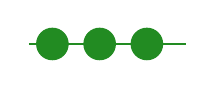
\begin{tikzpicture}
                \draw[ForestGreen, thick] (0,0) -- (2,0); % Bus
                \foreach \x in {0.3, 0.9, 1.5} {
                        \filldraw[ForestGreen] (\x, 0) circle (2mm);
                    }
            \end{tikzpicture}
            \caption{Bus}
        \end{subfigure}%
        % Ring Topology
        \begin{subfigure}[b]{0.25\textwidth}
            \centering
            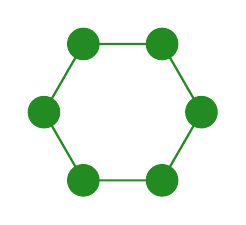
\begin{tikzpicture}
                \draw[ForestGreen, thick] (0:1cm) \foreach \x in {60,120,...,360} {
                        -- (\x:1cm)
                    } -- cycle; % Completes the circle
                \foreach \x in {0,60,...,300} {
                        \filldraw[ForestGreen] (\x:1cm) circle (2mm);
                    }
            \end{tikzpicture}
            \caption{Ring}
        \end{subfigure}
        % Stern
        \begin{subfigure}[b]{0.25\textwidth}
            \centering
            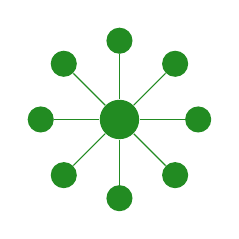
\begin{tikzpicture}
                \node[fill=ForestGreen, circle, minimum size=5mm] at (0,0) (center) {};
                \foreach \x in {0,45,...,315} {
                        \node[fill=ForestGreen, circle, minimum size=2mm] at (\x:1cm) (node\x) {};
                        \draw[ForestGreen] (center) -- (node\x);
                    }
            \end{tikzpicture}
            \caption{Stern}
        \end{subfigure}%
        % Mesh Topology
        \begin{subfigure}[b]{0.25\textwidth}
            \centering
            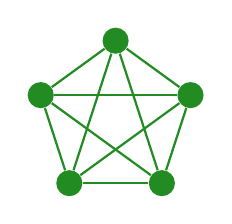
\begin{tikzpicture}
                % Define nodes
                \foreach \x [count=\i from 1] in {18,90,162,234,306} {
                        \node[fill=ForestGreen, circle, minimum size=2mm] at (\x:1cm) (node\i) {};
                    }

                % Connect nodes (to border points)
                \foreach \x in {1,2,3,4,5} {
                        \foreach \y in {\x,...,5} {
                                \ifnum\x=\y\relax
                                    % skip self-connection
                                \else
                                    \draw[ForestGreen, thick] (node\x) -- (node\y);
                                \fi
                            }
                    }

            \end{tikzpicture}
            \caption{Vollvermascht}
        \end{subfigure}
        \begin{subfigure}{.25\textwidth}
            \centering
            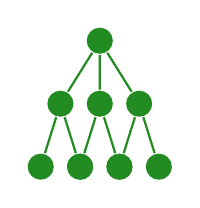
\begin{tikzpicture}[
                    sibling distance=5mm, % Adjust spacing between siblings
                    level distance=8mm, % Adjust spacing between parent and child nodes
                    every node/.style={fill=ForestGreen, circle, thick, minimum size=2mm},
                    edge from parent/.style={ForestGreen, thick, draw}
                ]
                % Define the tree
                \node {} % Root node
                child {node {}
                        child {node {}}
                        child {node {}}
                    }
                child {node {}
                        child {node {}}
                        child {node {}}
                    }
                child {node {}
                        child {node {}}
                        child {node {}}
                    };

            \end{tikzpicture}
            \caption{Baum}
        \end{subfigure}
        \caption{Beispiele von Netzwerk-Topologien}
        \label{fig:topologie}
    \end{figure}